
\documentclass{beamer}

\usepackage{algpseudocode, color, colortbl}

\usepackage{hyperref}
\hypersetup{
    colorlinks=true,
    urlcolor=blue,
}

\usetheme{Montpellier}
\usecolortheme{rose}

% page numbers, from
% https://tex.stackexchange.com/questions/137022/how-to-insert-page-number-in-beamer-navigation-symbols
\expandafter\def\expandafter\insertshorttitle\expandafter{%
  \insertshorttitle\hfill%
  \insertframenumber\,/\,\inserttotalframenumber}

\definecolor{Gray}{gray}{0.8}
\newcolumntype{g}{>{\columncolor{Gray}}c}

\newcommand{\stanza}{ \\~\ }

\title{05. Hash Tables}
\subtitle{CPSC 535 $\sim$ Spring 2019}
\author{Kevin A. Wortman}
\institute{ 
\includegraphics[height=2cm]{csuf-logo-cmyk} }
\date{February 25, 2019 \stanza

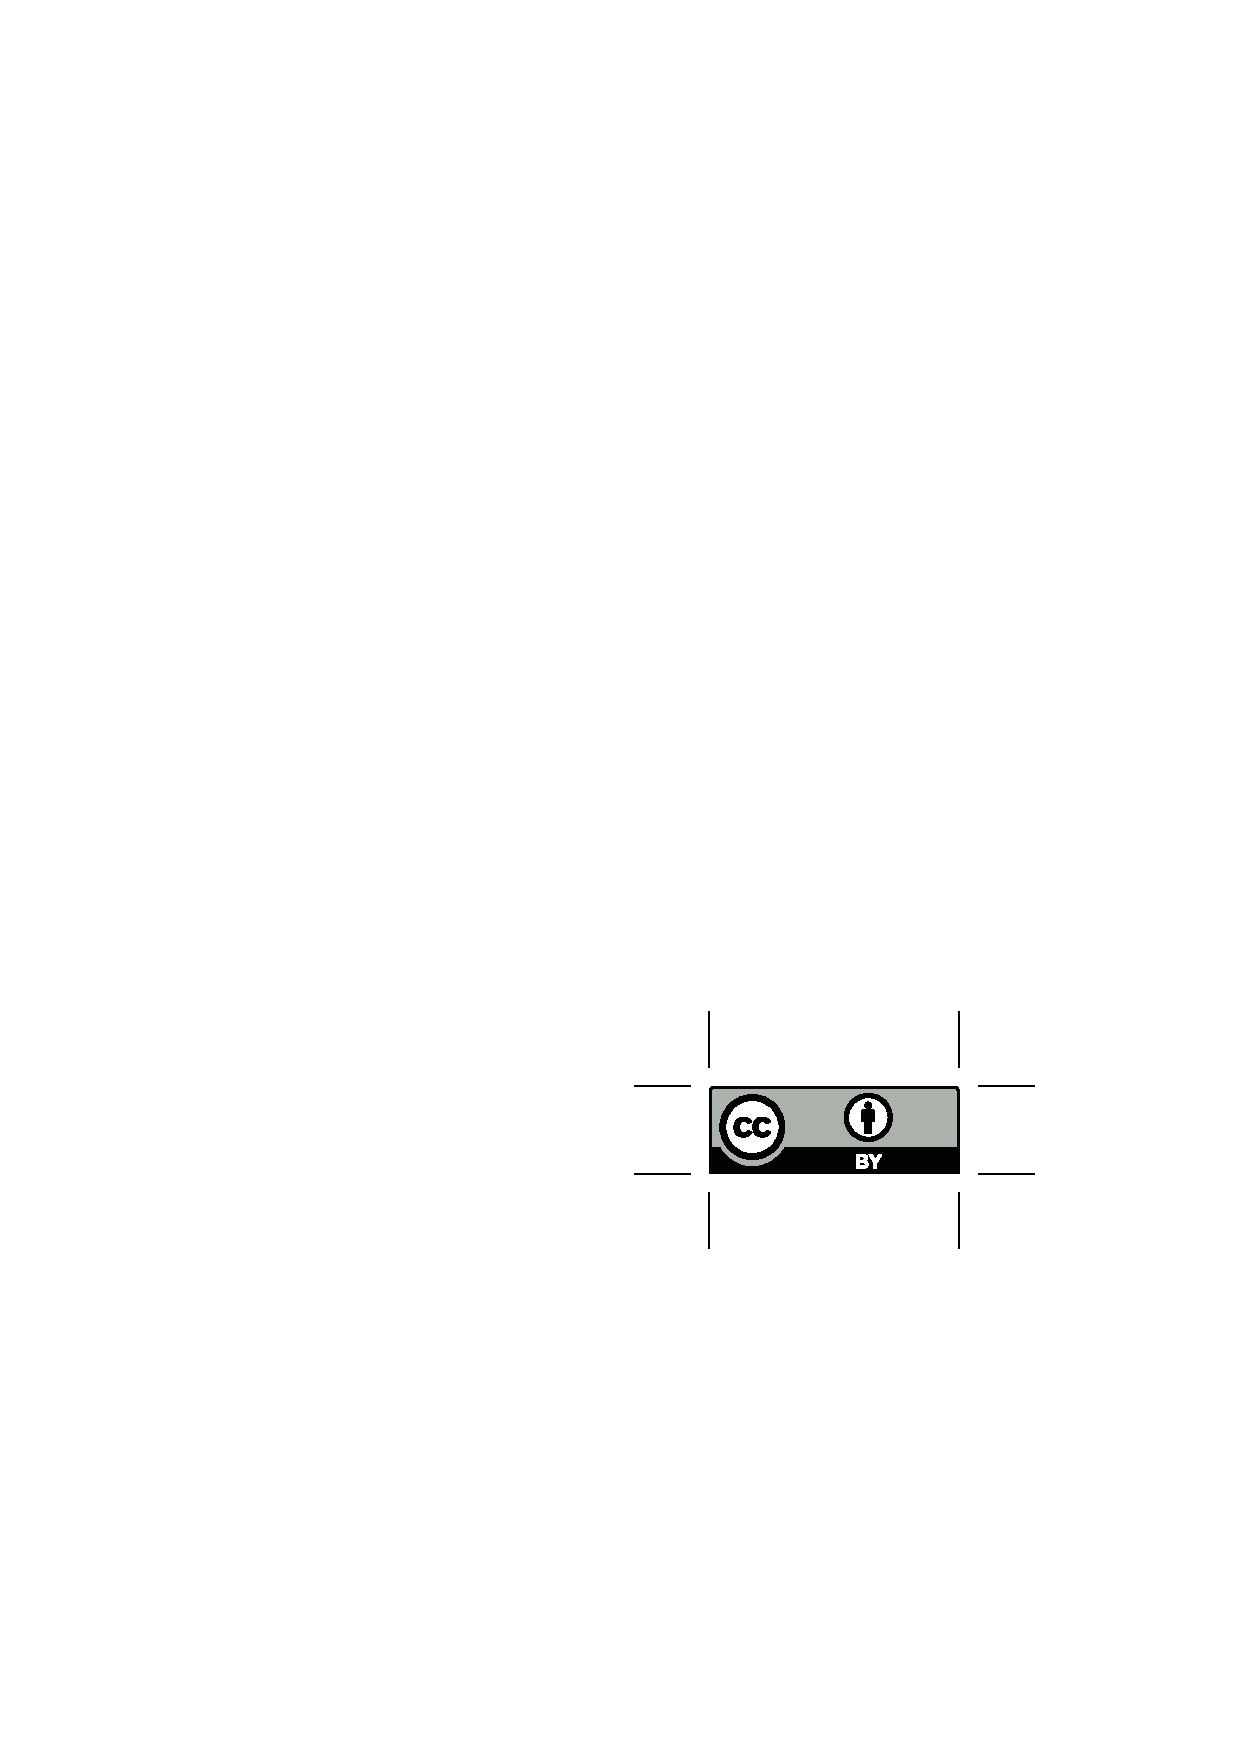
\includegraphics[height=14pt]{by} \\

{\tiny
This work is licensed under a
\href{http://creativecommons.org/licenses/by/4.0/}{Creative Commons Attribution 4.0 International License}.
}}

\begin{document}

\begin{frame}
  \titlepage
\end{frame}

\begin{frame} \frametitle{Big Idea in Algorithm Design}

Recall that radix sort takes $\Theta(n)$ time
\begin{itemize}
  \item linear time is extremely fast
  \item same asymptotically as merely observing all the elements
  \item under the assumptions of radix sort, sorting is ``free''; no significant
    computation time
\end{itemize}
\vspace{.5cm}
\textbf{Natural questions:}
\begin{itemize}
  \item How far can we take this?
  \item What is the most powerful way we can organize data, and still only spend
$O(1)$ time per element?
  \item What are the trade-offs (assumptions) and are they worth it?
\end{itemize}
\end{frame}

\begin{frame} \frametitle{The Story So Far}
\begin{itemize}
  \item \emph{offline:} all operations performed at once; e.g. BUILD-HEAP
  \item \emph{online:} data structure valid after each individual operation;
    e.g. DELETE-MIN
  \item computing order offline = sorting problem = $\Omega(n \log n)$ lower
    bound = $\Omega(\log n)$/element
  \item maintaining order online = search tree = $\Theta(\log n)$/element
  \item sorting \underline{integers} = radix sort = $\Theta(n)$ total =
    $\Theta(1)$/element; subjectively more complex
  \item Question: what about maintaining order \underline{of integers} online,
    $\Theta(1)$ per element?
\end{itemize}
\end{frame}

\begin{frame} \frametitle{Introducing Hash Tables}
\begin{itemize}
  \item (later) van Emde Boas trees can maintain order of integers in
    $\Theta(\log \log n)$ per element (huh?)
  \item (today) hash tables can't maintain order, but can support dictionary
    operations INSERT/SEARCH/DELETE, in $\Theta(1)$/element \textbf{expected} time
  \item hash tables match runtime of arrays, but (again) are more complicated
    to understand and implement
  \item success story for algorithm design
  \item mainstream; taken for granted in CS systems design
  \item GZIP, DNS, Java, Python, JSON, $\ldots$
\end{itemize}
\end{frame}

\begin{frame} \frametitle{Dictionary Operations}
CREATE($T$): intialize $T$ as a valid dictionary \stanza

INSERT($T, k, v$): associate key $k$ and value $v$ in dictionary $T$;
$k$ must not already be in $T$ \stanza

SEARCH($T, k$): return the value $v$ associated with key $k$ in dictionary $T$;
or return NIL if $k$ is absent from $T$ \stanza

DELETE($T, k$): remove key $k$ and its associated value from dictionary $T$;
$k$ must already be in $T$ \stanza

(Practical implementations are often more flexible about re-insertions and
inneffectual deletions.)
\end{frame}

\begin{frame} \frametitle{Direct Address Table}
Suppose the \emph{universe} of keys is $k \in U=\{0, 1, \ldots, m-1\}$ for
fixed $m$; create $m$-element array; $T[k]=v$ (or NIL if $k$ is absent)
\vspace{.5cm}
\begin{columns}
\begin{column}{0.5\textwidth}
  {\small

  \begin{algorithmic}[1]
    \Function{DA-CREATE}{T}
    \State $T[0 \ldots m-1] = $ NIL
    \EndFunction
  \end{algorithmic}

  \begin{algorithmic}[1]
    \Function{DA-INSERT}{T, k, v}
    \State $T[k] = v$
    \EndFunction
  \end{algorithmic}

  }

\end{column}
\begin{column}{0.5\textwidth}
  {\small

  \begin{algorithmic}[1]
    \Function{DA-SEARCH}{T, k}
    \State \Return{$T[k]$}
    \EndFunction
  \end{algorithmic}

  \begin{algorithmic}[1]
    \Function{DA-DELETE}{T, k}
    \State $T[k] = $ NIL
    \EndFunction
  \end{algorithmic}

  }
\end{column}
\end{columns}
\vspace{.5cm}
$\Theta(m)$ space; CREATE is $\Theta(m)$ time; rest are $\Theta(1)$ time;
good when $m \in O(n)$ but $m$ could be exponential in $n$
\end{frame}

\begin{frame} \frametitle{Hash Functions}
\begin{itemize}
  \item $U = $ set of keys, $m$ = size of array
  \item $m=|U|$ impractical in general
  \item introduce \emph{hash function} $h : U \mapsto \{0, 1, \ldots, m-1 \}$
  \item $h$ ``compresses'' large space of keys $U$ into denser space of table
    indices $\leq m$
  \item \emph{collisions} exist, i.e. $k_1, k_2 \in U$,
    $k_1 \ne k_2,$
    such that \[ h(k_1) = h(k_2) \]
    (pigeonhole principle)
  \item hard part is designing a concrete $h$, and collision resolution
    strategy
\end{itemize}
\end{frame}

\begin{frame} \frametitle{Collision Resolution by Chaining}
\textbf{Chaining:} each $T[i]$ is a linked list of (colliding) key-value entries
\vspace{.5cm}
\begin{columns}
\begin{column}{0.5\textwidth}
  {\small

  \begin{algorithmic}[1]
    \Function{CHAINED-CREATE}{T}
    \State $T[0 \ldots m-1] = $ empty list
    \EndFunction
  \end{algorithmic}

  \begin{algorithmic}[1]
    \Function{CHAINED-INSERT}{T, k, v}
    \State insert $(k, v)$ at front of $T[h(k)]$
    \EndFunction
  \end{algorithmic}
  }
\end{column}
\begin{column}{0.5\textwidth}
  {\small

  \begin{algorithmic}[1]
    \Function{CHAINED-SEARCH}{T, k}
    \State search for $k$ in $T[h(k)]$
    \EndFunction
  \end{algorithmic}

  \begin{algorithmic}[1]
    \Function{DA-DELETE}{T, k}
    \State remove $k$ from $T[h(k)]$
    \EndFunction
  \end{algorithmic}
  }
\end{column}
\end{columns}
\vspace{.5cm}
CREATE is $O(m)$; INSERT is $O(1)$; SEARCH and DELETE are $O(|T[h(k)]|)$
\end{frame}

\begin{frame} \frametitle{Chaining Analysis}
SEARCH, DELETE take $\Theta(n)$ time in worst case \stanza


Let $\alpha = n/m = $ average keys/table element = \textbf{load factor} \stanza

\textbf{simple uniform hashing assumption}: any element is equally likely to
hash to each index, independent of other elements \stanza

Under this assumption, expected chain length is $O(1+\alpha)$ \\
$\implies$ SEARCH, DELETE take $O(1+\alpha)$ expected time each \stanza

To achieve $O(1+\alpha)=O(1)$ exp. time, choose $m \in \Omega(n)$ \stanza

e.g. choose $m \geq 2n$ so
\[ \alpha = \frac{n}{m} \leq \frac{n}{(2n)} = \frac{1}{2} \]
\end{frame}

\begin{frame} \frametitle{Deterministic Hash Functions}
First: map keys to natural numbers $\{0, 1, \ldots \}$; \\
henceforth assume $k \in \mathbb{N}$ \stanza

\textbf{Division method:} $h(k) = k \mod m,$ \\
for appropriate $m$ \\
e.g. $m$ is a prime ``not too close to'' a power of 2 \stanza

\textbf{Multiplication method:} $h(k) = \big\lfloor m(kA - \lfloor kA \rfloor) \big\rfloor$ \\
for carefully-chosen $0<A<1$ \\
e.g. $A \approx (\sqrt{5} -1)/2$ \stanza

Each is fast, but deterministic, so an adversary could craft a set of keys
that force $\Theta(n)$/element $\implies \Theta(n^2)$ to insert $n$ elements
\end{frame}

\begin{frame} \frametitle{Hash Collision Exploits}
Denial-of-service attacks based on hash collisions are a real thing
\begin{itemize}
  \item \href{https://nvd.nist.gov/vuln/detail/CVE-2011-4885}{CVE-2011-4885}
  \item \href{https://www.exploit-db.com/exploits/18305}{working exploit}
\end{itemize}
\end{frame}

\begin{frame} \frametitle{Universal Hashing}
Goal: prevent hash collision exploit \stanza

Hash function not compiled in; picked randomly at runtime (once per boot,
execution, or table creation); unknowable to adversary \stanza

A set $\mathcal{H}$ of hash functions is \textbf{universal} when
\begin{itemize}
  \item for any distinct keys $k, l \in U,$
  \item the number of hash functions for which $k$ and $l$ collide,
    is at most
    \[ \frac{|\mathcal{H}|}{m} \]
  \item i.e. if $h$ is picked randomly from $\mathcal{H},$ then for \textbf{any} keys $k,l,$
    \[ Pr[h(k)=h(l)] = Pr[\text{two random table indices match}] = \frac{1}{m} \]
\end{itemize}
\end{frame}

\begin{frame} \frametitle{Universal Hashing Analysis}
\emph{Theorem:} If hash function $h$ is chosen randomly from a universal family;
$T$ is a chained hash table using $h,$
with $m$ table elements,
containing $n$ keys,
and with load factor $\alpha=n/m;$
$k$ is a query key that hashes to list $\ell$;
then the expected length of $\ell$ is $\alpha$ if $k \in T,$ or
$(1+\alpha)$ if $k \notin T.$ \stanza

\textbf{Note:} the hash function type and collision resolution algorithm need
to be analyzed together. \stanza

\emph{Corollary:} In a hash table using a universal hash function and chaining
collision resolution, INSERT takes $O(1)$ time, while SEARCH and DELETE each
take $O(1)$ expected time and $\Theta(n)$ worst-case time.
\end{frame}

\begin{frame} \frametitle{An Example Universal Hash Family}
Fix $p$ as a prime number greater than every possible key $k$ \stanza

Let $a, b$ be int. parameters with $1 \leq a < p$ and $0 \leq b < p$; define
\[ h_{ab}(k) \equiv ((ak + b) \mod p) \mod m . \]
Number theory shows this is a universal family. \stanza

Conveniences
\begin{itemize}
  \item can hardcode $p$ as a prime near $2^W-1$
  \item generating $h_{ab}$ only involves choosing two random int's $<p$
  \item evaluating $h_{ab}$ only involves one integer multiply, one add,
    and two modulo operations
  \item can recalibrate a fixed $h_{ab}$ to any $m$
\end{itemize}
\end{frame}

\begin{frame} \frametitle{Open Addressing}
Concern with chaining: linked lists have poor \emph{locality of reference},
require expensive allocate/free operations, and are conceptually complicated. \stanza

\textbf{open addressing:} all key-value entries are stored direclty in the table $T$ itself;
there are no chains \stanza

Modest assumptions
\begin{itemize}
  \item each $T[i]$ can store either an active $(k, v)$ entry; or NIL (meaning
    never used); or TOMBSTONE (meaning was once active, but is now empty)
  \item $n<m$, i.e. $\alpha<1$
\end{itemize}
\end{frame}

\begin{frame} \frametitle{Open Addressing Delete}
DELETE:
\begin{itemize}
  \item let $i=h(k);$ \textbf{probe} (examine) $T[i]$
  \item if $k$ is found, $T[i]=$ TOMBSTONE, done
  \item else if $T[i]$ is NIL, conclude $k \notin T,$ done
  \item else ($T[i]$ is TOMBSTONE or key other than $k$), probe a different index
  \item after $m$ probes, conclude $k \notin T,$ stop (otherwise infinite loop)
\end{itemize}
\vspace{.5cm}
\textbf{probe sequence}: sequence of indices probed; different approaches \stanza

$O(|\text{probe sequence}|)$ time
\end{frame}

\begin{frame} \frametitle{Open Addressing Search and Insert}
SEARCH:
\begin{itemize}
  \item probe in the same order as DELETE
  \item keep searching past TOMBSTONE elements
\end{itemize}
\vspace{.5cm}
INSERT:
\begin{itemize}
  \item probe in the same order as DELETE
  \item overwrite the first $T[i]$ containing NIL or TOMBSTONE
\end{itemize}
\end{frame}

\begin{frame} \frametitle{Probe Sequence Functions; Linear Probing}
Hash function: $h : U \mapsto \{0, 1, \ldots, m-1 \}$ \\
Probe sequence function:
$h : U \times \{0, 1, \ldots, m-1 \} \mapsto \{ 0, 1, \ldots, m-1 \}$,
i.e. \[ h(k, i) = i\text{th index to probe for key } k \]

\textbf{Linear probing:} probe in sequential order, so
\[ ps(k, i) = (h(k) + i) \mod m \]

Simple; excellent locality of reference; but develops long \textbf{clusters} of
occupied elements; an empty slot after $\ell$ occupied slots will be filled
with probability $(\ell+1)/m$
\end{frame}

\begin{frame} \frametitle{Quadratic Probing}
\textbf{Quadratic probing:}
\[ ps(k, i) = (h(k) + c_1 i + c_2 i^2) \mod m \]
for constant parameters $c_1, c_2$ (with some constraints)\stanza

Much less clustering than linear probing; but still some, because if $k_1, k_2$
collide because $h(k_1)=h(k_2)$, then their entire probe sequences collide. \stanza

$\implies$ partially mitigates the clustering problem; but the $ps$ function
is more expensive, and locality of reference is not as good
\end{frame}

\begin{frame} \frametitle{Double Hashing}
\textbf{Double hashing:}
\[ ps(k, k) = (h_1(k) + i \cdot h_2(k)) \mod m \]
where $h_1, h_2$ are two distinct hash functions \stanza

Since $h_1, h_2$ are different, even if $k_1,k_2$ collide at first with
$h_1(k_1)=h_1(k_2),$ their probe sequences are almost certainly different

$\implies$ clustering problem essentially solved; but more expensive than
linear/quadratic programming because we evaluate two hash functions, and
locality of reference is poor (random), though still entirely within $T$
\end{frame}

\begin{frame} \frametitle{Open Addressing Analysis}
\textbf{Universal hashing assumption:} the probability of every possible
probe sequence
$\langle p_1, p_2, \langle, p_m \rangle$
with each $p_i \in \{0, 1, \ldots, m_1 \}$
is equally likely. \stanza

\emph{Theorem:} Under the universal hashing assumption, an open-address hash
table with load factor $\alpha<1$ performing a search makes at most
\[ \frac{1}{\alpha} \ln \frac{1}{1-\alpha} \]
probes when the search succeeds, or at most
\[ \frac{1}{1-\alpha} \]
probes when the search fails.

\emph{Corollary:} Inserting requires at most $\frac{1}{1-\alpha}$ probes on average.

\emph{Corollary:} If $\alpha \in O(1)$ then the INSERT, SEARCH, and DELETE operations
on an open-addressing hash table each take $O(1)$ expected time and $O(m)=O(n)$
worst case time.
\end{frame}

\begin{frame} \frametitle{Perfect hashing}
\emph{Static hashing:} set of keys is known statically (algorithm design-time or
program compile-time)
\begin{itemize}
  \item CREATE, INSERT happen offline (all-at-once) at compile-time
  \item SEARCH happens online at run-time
  \item DELETE not supported
\end{itemize}

\textbf{Perfect hashing:} static hashing where SEARCH $O(1)$ worst case time
(\textbf{not} $O(1)$ expected time)

Applies when key set is constant, or evolves very slowly: top-level domains,
programming language keywords, state abbreviations (CA), etc.
\end{frame}

\begin{frame} \frametitle{Two-Level Hashing}
  \textbf{Hash-table-of-hash-tables:}
  \begin{itemize}
    \item \emph{outer} hash table w/ function $h$
    \item slot $T[j]$ holds an \emph{inner} table using function $h_j$
    \item all hash functions $h$, $h_j$ are universal
    \item if $T[j]$ holds $n_j$ colliding keys, then its size $m_j$ must be
      $\Omega(n_j^2)$
    \item non-obvious: large $n_j^2$ size prevents collisions in the inner
      tables but the whole table still only takes $O(n)$ space
  \end{itemize}
\end{frame}

\begin{frame} \frametitle{Two-Level Collisions}
\emph{Theorem:} if inner hash table $T[j]$ uses a universal hash function $h_j$
and has $m_j=n_j^2$, then the probability of a collision in $T[j]$ is less than $\frac{1}{2}$ \\
\emph{Sketch:} there are $\binom{n_j}{2}$ pairs of keys; due to universal $h_j$, each
collides with probability $\frac{1}{m}$; so
\[ E[\text{\# collisions}]
   = \binom{n_j}{2} \cdot \frac{1}{m_j}
   = \binom{n_j}{2} \cdot \big( \frac{1}{n_j^2} \big)
   = \big( \frac{n_j^2-n}{2} \big) \cdot \frac{1}{n_j^2}
   < \frac{1}{2}. \]

To pick an $h_j$, keep retrying until no collisions $\implies O(1)$ expected trials
\end{frame}

\begin{frame} \frametitle{Two-Level Analysis}
\emph{Theorem:} total space used by a two-level hash is $O(n)$ \\
\emph{Sketch:}
\begin{itemize}
  \item outer hash uses $O(n)$ space
  \item each $T[j]$ has $n_j$ elements and uses $\Theta(n_j^2)$; space
  \item $O(1)$ collisions in $T[j] \implies n_j \in O(1) \implies n_j^2 \in O(1)$
\end{itemize}
\vspace{.5cm}
\textbf{Takeaway:} two-level perfect hash table takes $O(n)$ expected time to
create statically; a SEARCH takes $O(1)$ deterministic worst-case time at runtime.
\end{frame}

\end{document}
